\documentclass[a4paper,12pt]{article}

%%% Работа с русским языком
\usepackage{cmap}					% поиск в PDF
\usepackage{mathtext} 				% русские буквы в формулах
\usepackage[T2A]{fontenc}			% кодировка
\usepackage[utf8]{inputenc}			% кодировка исходного текста
\usepackage[english,russian]{babel}	% локализация и переносы

%%% Дополнительная работа с математикой
\usepackage{amsmath,amsfonts,amssymb,amsthm,mathtools} % AMS
\usepackage{icomma} % "Умная" запятая: $0,2$ --- число, $0, 2$ --- перечисление

%% Номера формул
%\mathtoolsset{showonlyrefs=true} % Показывать номера только у тех формул, на которые есть \eqref{} в тексте.
%\usepackage{leqno} % Нумерация формул слева

%% Свои команды
\DeclareMathOperator{\sgn}{\mathop{sgn}}

%% Перенос знаков в формулах (по Львовскому)
\newcommand*{\hm}[1]{#1\nobreak\discretionary{}
{\hbox{$\mathsurround=0pt #1$}}{}}

%%% Работа с картинками
\usepackage{graphicx}  % Для вставки рисунков
\graphicspath{{materials}{images2/}}  % папки с картинками
\setlength\fboxsep{3pt} % Отступ рамки \fbox{} от рисунка
\setlength\fboxrule{1pt} % Толщина линий рамки \fbox{}
\usepackage{wrapfig} % Обтекание рисунков текстом

%%% Работа с таблицами
\usepackage{array,tabularx,tabulary,booktabs} % Дополнительная работа с таблицами
\usepackage{longtable}  % Длинные таблицы
\usepackage{multirow} % Слияние строк в таблице

%%% Теоремы
\theoremstyle{plain} % Это стиль по умолчанию, его можно не переопределять.
\newtheorem{theorem}{Теорема}[section]
\newtheorem{proposition}[theorem]{Утверждение}
 
\theoremstyle{definition} % "Определение"
\newtheorem{corollary}{Следствие}[theorem]
\newtheorem{problem}{Задача}[section]
 
\theoremstyle{remark} % "Примечание"
\newtheorem*{nonum}{Решение}

%%% Программирование
\usepackage{etoolbox} % логические операторы

%%% Страница
%\usepackage{extsizes} % Возможность сделать 14-й шрифт
\usepackage{geometry} % Простой способ задавать поля
	\geometry{top=25mm}
	\geometry{bottom=25mm}
	\geometry{left=20mm}
	\geometry{right=20mm}
 %

%%% Способ сделать тоже самое(но красивее:)
%\usepackage[margin=0.8in]{geometry}

 
\usepackage{fancyhdr} % Колонтитулы
 	\pagestyle{fancy}
 	\renewcommand{\headrulewidth}{0mm}  % Толщина линейки, отчеркивающей верхний колонтитул
 	\lfoot{}
 	\rfoot{}
 	\rhead{}
 	\chead{}
 	\lhead{ }
 	% \cfoot{Нижний в центре} % По умолчанию здесь номер страницы

\usepackage{setspace} % Интерлиньяж
%\onehalfspacing % Интерлиньяж 1.5
%\doublespacing % Интерлиньяж 2
%\singlespacing % Интерлиньяж 1

\usepackage{lastpage} % Узнать, сколько всего страниц в документе.

\usepackage{soulutf8} % Модификаторы начертания

\usepackage{hyperref}
\usepackage[usenames,dvipsnames,svgnames,table,rgb]{xcolor}
\hypersetup{				% Гиперссылки
    unicode=true,           % русские буквы в раздела PDF
    pdftitle={Заголовок},   % Заголовок
    pdfauthor={Автор},      % Автор
    pdfsubject={Тема},      % Тема
    pdfcreator={Создатель}, % Создатель
    pdfproducer={Производитель}, % Производитель
    pdfkeywords={keyword1} {key2} {key3}, % Ключевые слова
    colorlinks=true,       	% false: ссылки в рамках; true: цветные ссылки
    linkcolor=red,          % внутренние ссылки
    citecolor=green,        % на библиографию
    filecolor=magenta,      % на файлы
    urlcolor=blue           % на URL
}

%\renewcommand{\familydefault}{\sfdefault} % Начертание шрифта

\usepackage{multicol} % Несколько колонок

% Мои "дополнительные" пакеты
\usepackage{textcase} 
\usepackage{pdfpages}
\usepackage{amsmath}
\usepackage{titlesec}
\usepackage{floatrow}

\author{Подкидышев Алексей}
\title{Студент МФТИ ФИВТ - 1ый курс}
\date{\today}

%% Делаем красивый header:
\fancyhead[RO]{\footnotesize{\scshape\nouppercase{~\leftmark}}}
%% Делаем красивый header END

%Делаем большой отступ между section и subsection
\titlespacing*{\section} {0pt}{3.5ex plus 1ex minus .2ex}{2.7ex plus .2ex}
\titlespacing*{\subsection} {0pt}{2.7ex plus 1ex minus .2ex}{1ex plus .2ex}



\begin{document} % конец преамбулы, начало документа

\begin{center}
	\textit{\MakeTextUppercase{федеральное государственное автономное учреждение}}
		
	\vspace{0.5ex}
	
	\textbf{ \\ \MakeTextUppercase{<<Московский Физико-технический институт>>}}
\end{center}
\vspace{13ex}
\begin{flushright}
	\noindent
	{Александр Андреевич Харитонов,\\
	Подкидышев Алексей Сергеевич}
	\\
	\textit{Студенты факультета инноваций\\ и высоких технологий\\(группа 792)}
\end{flushright}
\begin{center}
	\vspace{23ex}
	\line(1,0){430}\\[4ex]
	{\LARGE\textbf{Лабораторная работа 1.2}}
	\vspace{2ex}
	
		
	\textbf{\large{<<Исследование эффекта Комптона>>}}\\[3ex]
	\line(1,0){430}\\[5ex]
	\vfill
	Долгопрудный 
	
	{\today}
\end{center}

\newpage
%\tableofcontents
\newpage
\renewcommand{\headrulewidth}{1pt}

\section{Описание работы}

\begin{minipage}{0.45\textwidth}
  
\subsection{Установка}
Блок схема установки изобрежена на рисунке. Источник излучения 1 служить цезий 137, испускающий $\gamma$ - лучи с энергией 662 кэВ. Он помещен в толстостенный свинцовый контейнер с коллиматором. Узкий пучок $\gamma$ - квантов попадает на графитовую мишень 2.

\begin{figure}[H]
        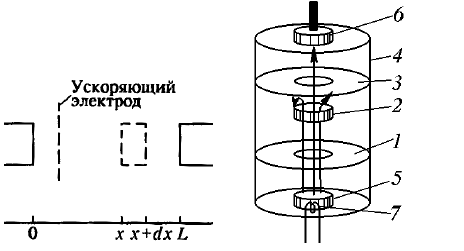
\includegraphics[width=0.89 \textwidth]{/pic1.png}
    \caption{Схема установки}
\end{figure}

\subsection{Теоритическая часть}

В составе рассеянного излучения, измеренного Комптоном, кроме исходной волны с частотой $\varpi_0$ появляется дополнительная длинноволновая компонента, отсутствующая в спектре первичного иззлучения. Появление этой компоненты легко объяснимо, если считать, что $\gamma$-излучение представляет собой поток квантов(фотонов), имеющих энергию $h \nu $ и импульс $p = \dfrac{\hbar \omega_0}{c}$.
Эффект Комптона — увеличение длины волны рассеянного излучения по сравнению с падающим — интерпретируется как результат упругого соударения двух частиц: фотона и свободного электрона. Изнчально $\gamma$ - квант имел начальную энергию $h \nu_0 $ и $\dfrac{\hbar \omega_0}{c}$ - импульс. После соударения электрон получит энергию $\gamma m c^2$ и импульс $\gamma m v,$ где $\gamma = \left(1 - \left(\frac{v}{c}\right)^2\right)^{-\frac{1}{2}},$ а $\gamma$ - квант рассеивается на некоторый угол. Его энергия и импульс соответсвенно $\hbar\omega_1, \frac{\hbar\omega_1}{c}.$\par

\end{minipage}
\hfill
\begin{minipage}{0.45\textwidth}
Из законов сохранения энергии и импульса нетрудно получить, что 
\[\Delta \lambda = \lambda_1 - \lambda_0 = \frac{h}{mc}(1 - \cos\theta) = \Lambda_K(1 - \cos\theta),\]
где $\Lambda_K = \frac{h}{mc} = 2,42\cdot10^{-10}\text{ см}$ называется комптоновской длиной волны электрона.\par
  
При рассеянии на связанных электронах изменение импульса кванта воспринимается атомом в целом. В силу того, что масса атома очень велика, не происходит заметной передачи энергии. Таким образом можно рассматривать такое рассеяние, как упругое соударние квантов с атомами. \par
Сечения комптоновского и томсоновского рассеяний по-разному зависят от энергии фотонов, поэтому эффект Комптона можно наблюдать наиболее отчетливо при использовании в качестве рассеивателя легких элементов и при энергии падающих лучей порядка сотен килоэлектрон-вольт.

\begin{figure}[H]
        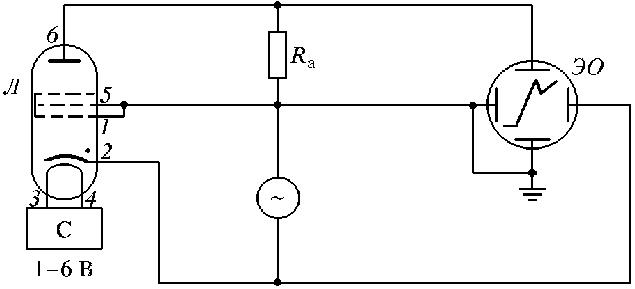
\includegraphics[width=0.89 \textwidth]{/pic2.png}
    \caption{Схема измерительного комплекса}
\end{figure}
\end{minipage}


\section{Ход Работы}

\begin{enumerate}
\item Настроили измерительные приборы
\item Записали результаты измерений
    
\begin{table}[H]
\begin{tabular}{|c|c|c|c|c|}
\hline
\rowcolor[HTML]{FFCE93} 
$\theta$ & $t$   & $N$  & $1/N, 10^-3 $ & $1 - \cos(\theta)$ \\ \hline
0     & 160 & 862 & 1,16009                     & 0                            \\ \hline
10    & 110 & 881 & 1,40845                     & 0,015192247                  \\ \hline
20    & 153 & 755 & 1,13507                     & 0,060307379                  \\ \hline
30    & 275 & 710 & 1,3245                      & 0,133974596                  \\ \hline
40    & 97  & 652 & 1,53374                     & 0,233955557                  \\ \hline
50    & 104 & 575 & 1,73913                     & 0,35721239                   \\ \hline
60    & 105 & 508 & 1,9685                      & 0,5                          \\ \hline
70    & 150 & 439 & 2,2779                      & 0,657979857                  \\ \hline
80    & 160 & 398 & 2,51256                     & 0,826351822                  \\ \hline
90    & 167 & 362 & 2,76243                     & 1                            \\ \hline
100   & 187 & 326 & 2,76243                     & 1,173648178                  \\ \hline
110   & 149 & 302 & 3,31126                     & 1,342020143                  \\ \hline
120   & 246 & 278 & 3,559712                    & 1,5                          \\ \hline
\end{tabular}
\caption{Таблица с измерениями}
\end{table}

\begin{minipage}{0.4\textwidth}
  \item На основании выражений для эффекта Комптона, а имено энергии отклонившихся гамма-квантов от угла, по изменению положения фотопиков сцинтилляционных мы можем определить энергию частиц на которых происходит отклонение.
\[ \dfrac{1}{N(\theta)} - \dfrac{1}{N(0)} = A(1 - \cos{\theta}) ,\] где $A$ - неизвестный коэффициент пропорциональности между $\epsilon (\theta)$ и номером канала $N (\theta)$, соответствующего вершине фотопика при указанном $\theta$. 
\[mc^2 = E(0) \dfrac{E(90)}{E(0) - E(90)} = E_\gamma \dfrac{N(0)}{N(0) - N(90)} \]
\end{minipage}
\hfill
\begin{minipage}{0.45\textwidth}
  \item Используя эксперементальные данные из таблицы 1, построим график по формуле, откладывая по оси абсцисс величину $(1 - \cos{\theta})$, а по оси ординат величину $\dfrac{1}{N}$.(см. Рис. 3)
\end{minipage}

\newpage
\item Посчитаем ошибку измерений

\begin{Large}
\[\Delta_{N_{90}} = 2,7\]
\[\Delta_{N_{0}} = 14,4\]
\[\Delta_{N_0 - N_{90}} = 17,1\]
\[\varepsilon_E = \sqrt{\left(\frac{\Delta_{N_{90}}}{N_{90}}\right)^2 + \left(\frac{\Delta_{N_0 - N_{90}}}{N_0 - N_{90}}\right)^2} = 0,39.\]
\end{Large}

\item
Вычислим энергию покоя частицы, на котолрой происходит комптоновское рассеивание первичных $\gamma$ - квантов:
\[mc^2 = E(0) \dfrac{E(90)}{E(0) - E(90)} = 480,8 \pm 18,8 \text{кэВ, где }  E_{\gamma} = 661,6 \text{ кэВ} .\]

\end{enumerate}

\begin{figure}[H]
        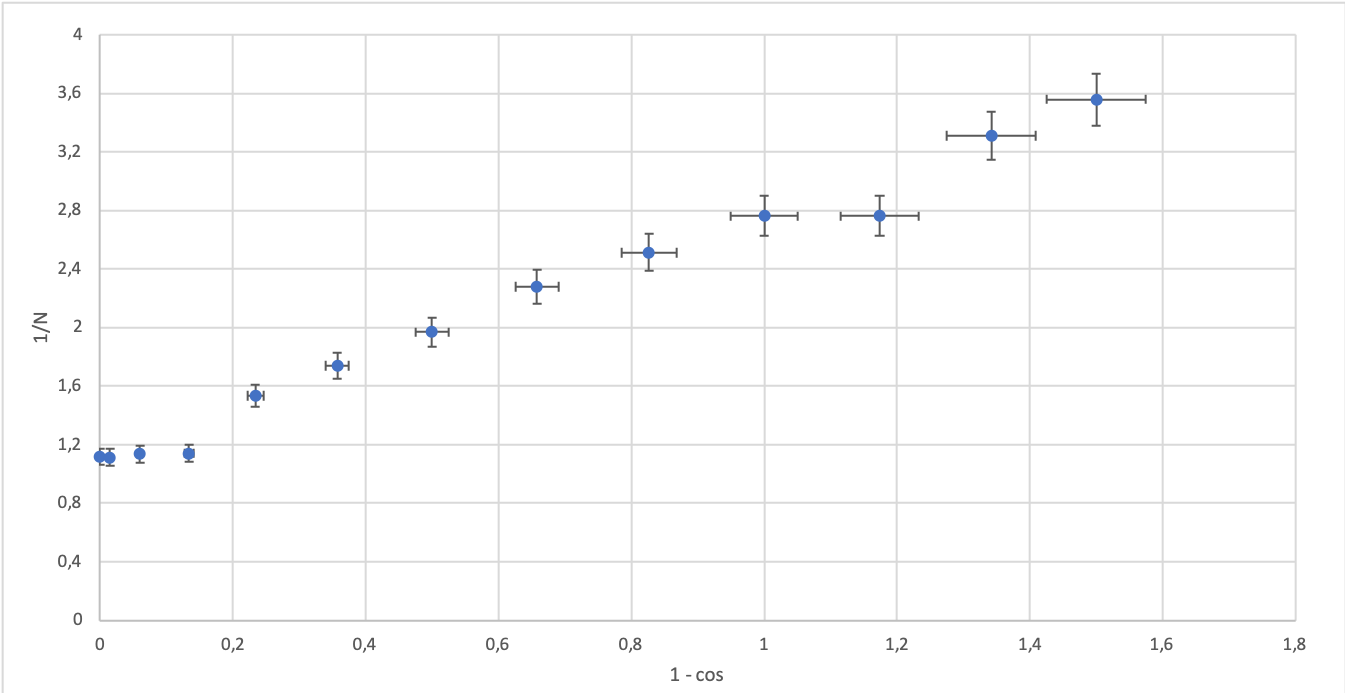
\includegraphics[width=0.9 \textwidth]{/graphics.png}
    \caption{График зависимости $\dfrac{1}{N}$ от $(1 - \cos(\theta)$}
\end{figure}

\section{Вывод}
\indent Мы исследовали энергетический спектр $\gamma$-квантов с помощью сцинтилляционного спектромет- ра, рассеянных на графите. Также определили энергию покоя частиц, на которых происходит комптоновское рассеяние : $E = 480, 8 \pm 18, 8 $ КэВ. Погрешность обуславливается возможным влиянием других работающих установок и неточное определение канала фотопика (наличие не бесконечно узкой ширины, вероятность для гамма-кванта совершить многократное рассеяние).
\end{document}